%%%%%%%%%%%%%%%%%%%%%%%%%%%%%%%%%%%%%%%%%
% The Legrand Orange Book
% LaTeX Template
% Version 3.1 (February 18, 2022)
%
% This template originates from:
% https://www.LaTeXTemplates.com
%
% Authors:
% Vel (vel@latextemplates.com)
% Mathias Legrand (legrand.mathias@gmail.com)
%
% License:
% CC BY-NC-SA 4.0 (https://creativecommons.org/licenses/by-nc-sa/4.0/)
%
% Compiling this template:
% This template uses biber for its bibliography and makeindex for its index.
% When you first open the template, compile it from the command line with the 
% commands below to make sure your LaTeX distribution is configured correctly:
%
% 1) pdflatex main
% 2) makeindex main.idx -s indexstyle.ist
% 3) biber main
% 4) pdflatex main x 2
%
% After this, when you wish to update the bibliography/index use the appropriate
% command above and make sure to compile with pdflatex several times 
% afterwards to propagate your changes to the document.
%
%%%%%%%%%%%%%%%%%%%%%%%%%%%%%%%%%%%%%%%%%

%----------------------------------------------------------------------------------------
%	PACKAGES AND OTHER DOCUMENT CONFIGURATIONS
%----------------------------------------------------------------------------------------

\documentclass[
	11pt, % Default font size, select one of 10pt, 11pt or 12pt
	fleqn, % Left align equations
	a4paper, % Paper size, use either 'a4paper' for A4 size or 'letterpaper' for US letter size
	%oneside, % Uncomment for oneside mode, this doesn't start new chapters and parts on odd pages (adding an empty page if required), this mode is more suitable if the book is to be read on a screen instead of printed
]{LegrandOrangeBook}

% Book information for PDF metadata, remove/comment this block if not required 
\hypersetup{
	pdftitle={Title}, % Title field
	pdfauthor={Author}, % Author field
	pdfsubject={Subject}, % Subject field
	pdfkeywords={Keyword1, Keyword2, ...}, % Keywords
	pdfcreator={LaTeX}, % Content creator field
}

\addbibresource{sample.bib} % Bibliography file

\definecolor{ocre}{RGB}{0,83,166} % Define the color used for highlighting throughout the book

\chapterimage{orange1.jpg} % Chapter heading image
\chapterspaceabove{8cm} % Default whitespace from the top of the page to the chapter title on chapter pages
\chapterspacebelow{8cm} % Default amount of vertical whitespace from the top margin to the start of the text on chapter pages

%----------------------------------------------------------------------------------------

\usepackage{tabularx} % For tabbing to a certain point
\usepackage{stmaryrd} % For \mapsfrom symbol
\usepackage{tikz}
\usetikzlibrary{matrix, positioning, arrows.meta} % <-- Add this line to enable matrix of math nodes

\newcommand{\End}[1]{\text{End}(#1)} % Endomorphism ring
\newcommand{\Hom}[2]{\text{Hom}(#1, #2)} % Hom-set
\renewcommand{\ker}[1]{\text{ker}(#1)} % Kernel of a linear map
\renewcommand{\Im}[1]{\text{Im}(#1)} % Image of a linear map
\renewcommand{\span}[1]{\text{span}(#1)} % Span of a set of vectors
\renewcommand{\bar}[1]{\overline{#1}} % Bar notation


\tikzset{%
    myarrow/.style = {-Stealth, shorten >=5pt}
}
\newcommand{\mypoint}[2]{\tikz[remember picture]{\node[inner sep=0, anchor=base](#1){$#2$};}}

\usepackage{mathtools} % for \xhookrightarrow

% For quotes
\usepackage{epigraph}

%----------------------------------------------------------------------------------------

\begin{document}

\chapterimage{UST.jpg} % Chapter heading image
%----------------------------------------------------------------------------------------
%	TITLE PAGE
%----------------------------------------------------------------------------------------

\titlepage % Output the title page
	% {
\includegraphics[width=\paperwidth]{background.pdf}} % Code to output the background image, which should be the same dimensions as the paper to fill the page entirely; leave empty for no background image
	{ % Title(s) and author(s)
		\centering\sffamily % Font styling
		\vspace{3cm}
		{\huge\color{ocre} Honors in Linear and Abstract Algebra\par} % Book title
		\vspace{2cm} % Vertical whitespace
		{Lecture Notes for MATH 2131\par} % Subtitle
		\vfill
		% \vspace{24pt} % Vertical whitespace
		% {\huge\bfseries \par} % Author name
	}

%----------------------------------------------------------------------------------------
%	COPYRIGHT PAGE
%----------------------------------------------------------------------------------------

\thispagestyle{empty} % Suppress headers and footers on this page

~\vfill % Push the text down to the bottom of the page

\noindent Copyright \copyright\ 2025 \\ % Copyright notice

\noindent \textsc{Published by Publisher}\\ % Publisher

\noindent \textsc{book-website.com}\\ % URL

\noindent Licensed under the Creative Commons Attribution-NonCommercial 3.0 Unported License (the ``License''). You may not use this file except in compliance with the License. You may obtain a copy of the License at \url{http://creativecommons.org/licenses/by-nc/3.0}. Unless required by applicable law or agreed to in writing, software distributed under the License is distributed on an \textsc{``as is'' basis, without warranties or conditions of any kind}, either express or implied. See the License for the specific language governing permissions and limitations under the License.\\ % License information

\noindent \textit{First printing, September 2025} % Printing/edition date

%----------------------------------------------------------------------------------------
%	TABLE OF CONTENTS
%----------------------------------------------------------------------------------------

\pagestyle{empty} % Disable headers and footers for the following pages

\tableofcontents % Output the table of contents

\cleardoublepage % Start the following content on a new page

\pagestyle{fancy} % Enable default headers and footers again

\newpage

\noindent {\Large \bf \sffamily Prefaces}

\vspace{8pt}

\noindent This lecture notes was written by a student in the course MATH 2131 -- Honors in Linear and Abstract Algebra by Professor Meng Guowu in HKUST. 

\noindent All diagrams in this lecture notes are written in LaTeX TikZ code.

\cleardoublepage % Start the following content on a new page

%----------------------------------------------------------------------------------------
%	SECTIONING EXAMPLES CHAPTER
%----------------------------------------------------------------------------------------

\chapterspaceabove{8cm} % Whitespace from the top of the page to the chapter title on chapter pages
\chapterspacebelow{8cm} % Amount of vertical whitespace from the top margin to the start of the text on chapter pages

%----------------------------------------------------------------------------------------
%	CHAPTER 1
%----------------------------------------------------------------------------------------
\chapter{Abstract Linear Spaces}

\epigraph{``I assume you have learnt linear algebra.''}{Guowu Meng}

\section{Binary Operation}\index{Binary Operation}

\begin{definition}[Binary Operation]
    A \emph{binary operation} on a set $S$ is a mapping of the elements of the Cartesian product $S \times S$ to $S$.
    \[ \begin{split}
            f : S \times S & \to S \\ (x,y) &\mapsto f(x,y)
        \end{split}\]
\end{definition}

\begin{example}
    A common example of a binary operation is addition on the set of natural numbers $\mathbb{N}$.
    \begin{equation}
        \begin{split}
            + : \mathbb{N} \times \mathbb{N} & \to \mathbb{N} \\ (x,y) &\mapsto x+y
        \end{split}
    \end{equation}
\end{example}

\begin{definition}[Associative Operation]
    A binary operation $f: S \times S \to S$ is said to be \emph{associative} if, for all $x,y,z \in S$, 
    \[ f(x,f(y,z)) = f(f(x,y),z) \]
\end{definition}

\begin{example}
    A common example of an associative (binary) operation is addition on the set of natural numbers $\mathbb{N}$. For all $x,y,z \in \mathbb{N}$, we have $x + (y + z) = (x + y) + z$.
\end{example}

\newpage

\begin{definition}[Identifiable Operation]
    A binary operation $f: S \times S \to S$ is said to be \emph{identifiable}, or \emph{unital}, if there exists an element $e \in S$, the \emph{identity} or \emph{unit element}, such that, for all $x \in S$
    \[ f(e,x) = x = f(x,e) \]
\end{definition}

\begin{example}
    A common example of an identifiable (binary) operation is multiplication on the set of natural numbers $\mathbb{N}$. The identity element is $1$, and for all $x \in \mathbb{N}$, we have $x \cdot 1 = x = 1 \cdot x$.
\end{example}

\begin{proposition}
    The identity element of an identifiable operation is unique.
\end{proposition}

\begin{proof}
    Let $e_1$ and $e_2$ be two identity elements for the operation $f$. Then, for any element $x \in S$, we have:
    \[ f(x,e_1) = x = f(e_1,x) \]
    \[ f(x,e_2) = x = f(e_2,x) \]
    Now, consider the element $e_1$:
    \[ f(e_1,e_2) = e_1 \]
    But since $e_2$ is an identity element, we also have:
    \[ f(e_1,e_2) = e_2 \]
    Therefore, we conclude that $e_1 = e_2$, proving the uniqueness of the identity element.
\end{proof}

\begin{remark}
    Two-sided identity must be unique, but one-sided identities need not be.
\end{remark}

\begin{example}
    Consider a set $X = \left\{ \begin{bmatrix}
        1 & a \\
        0 & 0 
    \end{bmatrix} \; \middle| \; a \in \mathbb{R} \right\}$ with the binary operation defined as matrix multiplication. This set has many left identity elements, but no two-sided identity element.
\end{example}

\begin{definition}[Inverse Operation]
    A binary operation $f: S \times S \to S$ is said to be \emph{invertible} if, for every element $x \in S$, there exists an element $y \in S$, called the two-sided \emph{inverse} of $x$, denoted as $x^{-1}$, such that
    \[ f(x,y) = e = f(y,x) \]
    where $e$ is the identity element of the operation.
\end{definition}

\begin{remark}
    Invertible operation exists if inverse operation exists, i.e., there exists an identity element.
\end{remark}

\begin{example}
    A common example of an invertible (binary) operation is addition on the set of integers $\mathbb{Z}$. For every integer $x \in \mathbb{Z}$, there exists an integer $y = -x$ such that:
    \begin{equation}
        x + (-x) = 0 = (-x) + x
    \end{equation}
    where $0$ is the identity element for addition.
\end{example}

\newpage

\begin{proposition}
    The inverse element of an invertible operation is unique.
\end{proposition}

\begin{proof}
    Let $y_1$ and $y_2$ be two inverses of an element $x \in S$. Then, by definition of inverse, we have:
    \[ f(x,y_1) = e = f(y_1,x) \]
    \[ f(x,y_2) = e = f(y_2,x) \]
    Now, consider the element $y_1$:
    \[ f(y_1,x) = e \]
    But since $y_2$ is also an inverse of $x$, we can substitute $e$ with $f(x,y_2)$:
    \[ f(y_1,x) = f(x,y_2) = e \]
    By the associativity of the operation, we can rearrange this to:
    \[ y_1 = f(y_1, e) = f(y_1,f(x,y_2)) = f(f(y_1,x),y_2) = f(e,y_2) = y_2 \]
    Thus, the inverse element is unique.
\end{proof}

\begin{definition}[Commutative Operation]
    A binary operation $f: S \times S \to S$ is said to be \emph{commutative} if, for all $x,y \in S$, the following holds:
    \[ f(x,y) = f(y,x) \]
\end{definition}

\begin{example}
    A common example of a commutative operation is addition on the set of integers $\mathbb{Z}$. For all $x,y \in \mathbb{Z}$, we have:
    \[ x + y = y + x \]
\end{example}

\begin{definition}[Distributive Operation (Harmonic Property)]
    A binary operation $g: S \times S \to S$ is said to be \emph{distributive} with respect to another binary operation $f: S \times S \to S$ if, for all $x,y,z \in S$, the following holds:
    \[ \begin{split}
        g(x,f(y,z)) &= f(g(x,y),g(x,z)) \\
        g(f(y,z),x) &= f(g(y,x),g(z,x))
    \end{split} \]
\end{definition}

\begin{example}
    A common example of a distributive operation is multiplication over addition on the set of integers $\mathbb{Z}$. For all $x,y,z \in \mathbb{Z}$, we have:
    \[ \begin{split}
        x \cdot (y + z) &= x \cdot y + x \cdot z \\
        (y + z) \cdot x &= y \cdot x + z \cdot x
    \end{split} \]
\end{example}

\newpage

\section{Groups, Rings, Fields}\index{Groups, Rings, Fields}

\begin{definition}[Monoid]
    A \emph{monoid} is a set $M$ equipped with a binary operation $f: M \times M \to M$ such that the following properties hold:
    \begin{enumerate}
        \item \emph{Closure Property:} For all $x,y \in M$, $f(x,y) \in M$.
        \item \emph{Associative Property}
        \item \emph{Identifiable Property}
    \end{enumerate}
    We say $(M, f)$ is a monoid, and $f$ is the \emph{monoid operation} on the set $M$. A set $M$ with a monoid operation $f$ is the \emph{monoid structure}.
\end{definition}

\begin{definition}[Group]
    A \emph{group} is a set $G$ equipped with a monoid operation $f: G \times G \to G$ with the additional property that every element has an inverse, \emph{Invertible Property}.
\end{definition}

\begin{example}
    $(\mathbb{R}\setminus\{0\}, \times)$ is a group, but $(\mathbb{R}, \times)$ is not a group since $0$ does not have a multiplicative inverse.
\end{example}

\begin{definition}[Abelian Monoid / Group]
    A monoid / group $(G, f)$ is said to be an \emph{abelian monoid / group} if the monoid / group operation $f$ is commutative, \emph{Commutative Property}.
\end{definition}

\begin{definition}[Unital Ring]
    A (unital) ring is a set $R$ equipped with two binary operations $f: R \times R \to R$ (addition) and $g: R \times R \to R$ (multiplication) such that the following properties hold:
    \begin{enumerate}
        \item \emph{Additive Group:} $(R, f)$ is an abelian group.
        \item \emph{Multiplicative Monoid:} $(R, g)$ is a monoid.
        \item \emph{Distributive Property:} $g$ with respect to $f$.
    \end{enumerate}
\end{definition}

\begin{definition}[Commutative Ring]
    A \emph{commutative ring} is a unital ring $R$ such that the multiplication operation $g: R \times R \to R$ is commutative.
\end{definition}

\begin{example}
    $(\mathbb{Z}, +, \times)$ is a unital commutative ring.
\end{example}

\begin{definition}[Field]
    A \emph{field} is a unital commutative ring $F$ such that every non-zero element has a multiplicative inverse.
\end{definition}

\begin{example}
    $(\mathbb{Q}, +, \times)$, $(\mathbb{R}, +, \times)$ and $(\mathbb{C}, +, \times)$ are fields.
\end{example}

\begin{example}
    $(\mathbb{Z}/2\mathbb{Z}, +, \times)$ is a field, where $\mathbb{Z}/2\mathbb{Z} = \{\bar{0}, \bar{1}\}$, $\bar{0}$ is the set of even integers and $\bar{1}$ is the set of odd integers.
    It follows the additions and multiplications below:
    \begin{equation}
        \begin{array}{c|cc}
              + & \bar{0} & \bar{1} \\ \hline
            \bar{0} & \bar{0} & \bar{1} \\
            \bar{1} & \bar{1} & \bar{0}
        \end{array}
        \quad
        \begin{array}{c|cc}
              \times & \bar{0} & \bar{1} \\ \hline
            \bar{0} & \bar{0} & \bar{0} \\
            \bar{1} & \bar{0} & \bar{1}
        \end{array}
    \end{equation}
\end{example}

\newpage

\section{Morphisms}\index{Morphisms}

\begin{definition}[Morphisms]
    A \emph{morphism} is a structure-preserving map between two algebraic structures (e.g., groups, rings, fields). Formally, let $(A, \cdot_A)$ and $(B, \cdot_B)$ be two algebraic structures. A morphism $f: A \to B$ is a set map / function such that:
    \[
        f(x \cdot_A y) = f(x) \cdot_B f(y) \quad \forall x, y \in A
    \]
\end{definition}

\begin{definition}[Monoid Homomorphism]
    A \emph{monoid homomorphism} is a morphism between two monoids that preserves the monoid structure. Formally, let $(M_1, \cdot_1)$ and $(M_2, \cdot_2)$ be two monoids with identity elements $e_1$ and $e_2$, respectively. A function $f: M_1 \to M_2$ is a monoid homomorphism if:
    \begin{enumerate}
        \item $f(x \cdot_1 y) = f(x) \cdot_2 f(y) \quad \forall x, y \in M_1$
        \item $f(e_1) = e_2$
    \end{enumerate}
\end{definition}

\begin{definition}[Group Homomorphism]
    A \emph{group homomorphism} is a morphism between two groups that preserves the group structure. Formally, let $(G_1, \cdot_1)$ and $(G_2, \cdot_2)$ be two groups with identity elements $e_1$ and $e_2$, respectively. A function $f: G_1 \to G_2$ is a group homomorphism if:
    \begin{enumerate}
        \item $f(x \cdot_1 y) = f(x) \cdot_2 f(y) \quad \forall x, y \in G_1$
        \item $f(e_1) = e_2$
        \item $f(x^{-1}) = (f(x))^{-1} \quad \forall x \in G_1$
    \end{enumerate}
\end{definition}

\begin{proposition}
    The second and third properties of a group homomorphism are consequences of the first property.
\end{proposition}

\begin{proof}
    Let $f: G_1 \to G_2$ be a group homomorphism satisfying the first property. We will show that the second and third properties follow from it.

    \textbf{Second Property:} To show that $f(e_1) = e_2$, we use the fact that $e_1$ is the identity element in $G_1$. For any element $x \in G_1$, we have:
    \[
        f(x) = f(x \cdot_1 e_1) = f(x) \cdot_2 f(e_1)
    \]
    The equation above holds for all $x \in G_1$. So for any $f(x) \in G_2$, this implies that $f(e_1)$ must be the identity element in $G_2$, i.e., $f(e_1) = e_2$.

    \textbf{Third Property:} To show that $f(x^{-1}) = (f(x))^{-1}$ for all $x \in G_1$, we use the fact that $x^{-1}$ is the inverse of $x$ in $G_1$. We have:
    \[
        e_2 = f(e_1) = f(x \cdot_1 x^{-1}) = f(x) \cdot_2 f(x^{-1})
    \]
    This shows that $f(x^{-1})$ is the inverse of $f(x)$ in $G_2$, i.e., $f(x^{-1}) = (f(x))^{-1}$.

    Therefore, both the second and third properties of a group homomorphism are indeed consequences of the first property.
\end{proof}

\begin{remark}
    For monoid homomorphisms, the second property cannot be derived from the first property. Consider the identity element $e_1$ in $M_1$. If we apply the first property, we get $f(e_1 \cdot_1 e_1) = f(e_1) \cdot_2 f(e_1)$. This simplifies to $f(e_1) = f(e_1) \cdot_2 f(e_1)$, which does not necessarily imply that $f(e_1)$ is the identity element in $M_2$, i.e., $f(e_1) \neq e_2$, but $f(e_1)$ is the idempotent element in $M_2$. Therefore, the second property must be explicitly stated for monoid homomorphisms.

    However in the case of group homomorphisms, the existence of inverses ensures that there is only one element that can be idempotent under the group operation, which is the identity element. Thus, for group homomorphisms, the second property can be derived from the first property.
\end{remark}

\begin{definition}[Ring Homomorphism]
    A \emph{ring homomorphism} is a morphism between two rings that preserves both the additive and multiplicative structures. Formally, let $(R_1, +_1, \cdot_1)$ and $(R_2, +_2, \cdot_2)$ be two rings with identity elements $0_1$, $1_1$ and $0_2$, $1_2$, respectively. A function $f: R_1 \to R_2$ is a ring homomorphism if:
    \begin{enumerate}
        \item $f(x +_1 y) = f(x) +_2 f(y) \quad \forall x, y \in R_1$
        \item $f(x \cdot_1 y) = f(x) \cdot_2 f(y) \quad \forall x, y \in R_1$
        \item $f(1_1) = 1_2$
    \end{enumerate}    
\end{definition}

\begin{definition}[Endomorphism]
    An \emph{endomorphism} is a morphism from an algebraic structure to itself. Formally, let $(A, \cdot)$ be an algebraic structure. An endomorphism $f: A \to A$ is a set map such that:
    \[
        f(x \cdot y) = f(x) \cdot f(y) \quad \forall x, y \in A
    \]
\end{definition}

\begin{definition}[Hom-set]
    The set of all morphisms from an algebraic structure $A$ to another algebraic structure $B$ is called the \emph{hom-set}, denoted by $\Hom{A}{B}$. 
\end{definition}

\begin{definition}[Endomorphism Ring]
    The set of all endomorphisms of an abelian group $(A, +)$, denoted by $\End{A}$, forms a (non-commutative) ring under pointwise addition and composition of set maps. The addition and multiplication operations are defined as follows:
    \[
        \begin{split}
            + : \End{A} \times \End{A} &\to \End{A} \\
            (f,g) &\mapsto (f+g: x \mapsto f(x) + g(x)) \qquad &f + g : A \to A \\ \\
            \circ : \End{A} \times \End{A} &\to \End{A} \\
            (f,g) &\mapsto (f \circ g: x \mapsto f(g(x))) \qquad &f \circ g : A \to A
        \end{split}
    \]
    The identity element for addition is the zero endomorphism, which maps every element to the identity element of the group. 
    \[ \begin{split}
        0: A &\to A \\
        x &\mapsto 0
    \end{split}
    \]
    The identity element for multiplication is the identity endomorphism, which maps every element to itself. 
    \[
    \begin{split}
        1: A &\to A \\
        x &\mapsto x
    \end{split}
    \]
    Note that all endomorphisms in $\End{A}$ are group homomorphisms and $\End{A} = \Hom{A}{A}$.
\end{definition}

\newpage

\section{Vector Spaces}\index{Vector Spaces}

\begin{definition}[Linear Structure]
    A \emph{linear structure} over a field $F$ on a set $V$ is a pair $(+, \cdot)$ where $(V, +)$ is an abelian group with a ring homomorphism $F \to \End{V}$, where $\End{V}$ is the endomorphism ring of the abelian group $(V, +)$.
    \[ \begin{split}
            \cdot : F &\to \End{V} \\
            \alpha &\mapsto (\alpha\cdot : \vec{x} \mapsto \alpha \vec{x}) \qquad \alpha \cdot : V \to V
        \end{split}
    \]
    The ring homomorphism is a (ring) action of the field $F$ on the abelian group $(V, +)$, called \emph{scalar multiplication}. The ring action can be written as a binary operation:
    \[
        \begin{split}
            \cdot : F \times V &\to V \\
            (\alpha, \vec{x}) &\mapsto \alpha \vec{x}
        \end{split}
    \]
\end{definition}

\begin{definition}[Linear Spaces / Vector Spaces]
    A linear space / vector space is a set with a linear structure over a field on the set.
\end{definition}

\begin{corollary}[Linear Spaces]
    A linear space over a field $F$ is a set $V$ equipped with two operations: vector addition $+: V \times V \to V$ and scalar multiplication $\cdot : F \times V \to V$, satisfying the following axioms for all $\vec{u}, \vec{v}, \vec{w} \in V$ and $\alpha, \beta \in F$:
    \begin{center}
        \begin{tabularx}{\textwidth}{XX}
            \toprule
            \textbf{Axiom} & \textbf{Statement} \\
            \midrule
            1. Associativity of addition & $(\vec{u} + \vec{v}) + \vec{w} = \vec{u} + (\vec{v} + \vec{w})$ \\
            2. Existence of additive identity & $\exists \vec{0} \in V$ such that $\forall \vec{u} \in V$, $\vec{u} + \vec{0} = \vec{u}$ \\
            3. Existence of additive inverses & $\forall \vec{u} \in V$, $\exists -\vec{u} \in V$ such that $\vec{u} + (-\vec{u}) = \vec{0}$ \\
            4. Commutativity of addition & $\vec{u} + \vec{v} = \vec{v} + \vec{u}$ \\
            5. Distributivity of scalar multiplication with respect to vector addition & $\alpha (\vec{u} + \vec{v}) = \alpha \vec{u} + \alpha \vec{v}$ \\
            6. Distributivity of scalar multiplication with respect to field addition & $(\alpha + \beta) \cdot = \alpha \cdot + \beta \cdot$ \\
            7. Compatibility of scalar multiplication with field multiplication & $(\alpha \beta) \cdot = (\alpha \cdot) \circ (\beta \cdot)$ \\
            8. Identity element of scalar multiplication & $F \ni 1 = (1\cdot : x \mapsto x) \in \End{V}$ \\
            \bottomrule
        \end{tabularx}
    \end{center}
\end{corollary}

\begin{remark}
    Note that the first four axioms ensure that $(V, +)$ is an abelian group, while the fifth axiom describes the endomorphism structure and the last three axioms describe the ring homomorphism.
\end{remark}

\begin{example}
    $F$ is a linear space over itself with the usual addition and multiplication operations.
    \[
        \begin{split}
            \cdot : F \times F &\to F \\
            (\alpha,\beta) &\mapsto \alpha \beta
        \end{split}
    \]
    The first $F$ is the field acting on the second $F$, which is the abelian group.
\end{example}

\begin{example}
    Let $X$ be a set and $F$ be a field. ($f$ is a set map)
    \[
    \begin{split}
        F[[X]] = \text{Map}(X, F) &\overset{\mathrm{def}}{=\joinrel=} \text{the set of all $F$-valued functions on } X \\
        &=\joinrel= \left\{ f : X \to F \right\}
    \end{split}
    \]
    $F[[X]]$ is a linear space over $F$ with the following operations defined pointwisely:
    \[
        \begin{split}
            + : F[[X]] \times F[[X]] &\to F[[X]] \\
            (f,g) &\mapsto (f+g: x \mapsto f(x) + g(x)) \qquad f + g : X \to F \\ \\
            \cdot : F \times F[[X]] &\to F[[X]] \\
            (\alpha,f) &\mapsto (\alpha f: x \mapsto \alpha f(x)) \qquad \alpha f : X \to F
        \end{split}
    \]
\end{example}

\begin{example}
    Let $X$ be a set and $F$ be a field.
    \[
        \begin{split}
            F[X] = \text{Map}_{\text{fin}}(X, F) &\overset{\mathrm{def}}{=\joinrel=} \text{the set of all finitely supported $F$-valued functions on } X \\
            &=\joinrel= \left\{ f : X \to F \mid f \text{ is finitely supported} \right\}
        \end{split}
    \]
    $F[X]$ is a linear space over $F$ as $F[X] \subseteq F[[X]]$ and the operations are defined pointwisely as in the previous example.

    $f: X \to F$ is finitely supported if the set $\{ x \in X \mid f(x) \neq 0 \}$ is finite or $f(x) \neq 0$ for only finitely many $x \in X$.
\end{example}

\begin{example}
    Let $t$ be a formal variable. Then $F[[t]] \overset{\mathrm{def}}{=\joinrel=} F[[\{ 1, t, t^2, \cdots \}]] = \sum_{n = 0}^{\infty} a_n t^n$ is the set of all formal power series in $t$ with coefficients in $F$ and $F[t] \overset{\mathrm{def}}{=\joinrel=} F[\{ 1, t, t^2, \cdots \}] = \sum_{n = 0}^{N} a_n t^n$ is the set of all polynomials in $t$ with coefficients in $F$. Both $F[[t]]$ and $F[t]$ are linear spaces over $F$.
\end{example}

\begin{example}
    Let $n$ be a positive integer and $F$ be a field. Then 
    \[
        F^n \overset{\mathrm{def}}{=\joinrel=} \left\{ 
        \begin{bmatrix}
        c_1 \\
        \vdots \\
        c_n
        \end{bmatrix}
        \;\middle|\; c_i \in F
        \right\}
    \]
    is the set of all \emph{column matrices} with $n$ entries in $F$. Elements in $F^n$ are written as $\vec{x}$ and are called \emph{column vectors}. $F^n$ is a linear space over $F$ with the following operations defined entrywisely:
    \[
        \begin{split}
            + : F^n \times F^n &\to F^n \\
            (\vec{a}, \vec{b}) &\mapsto \vec{a} + \vec{b} = \begin{bmatrix}
            a_1 + b_1 \\
            \vdots \\
            a_n + b_n
            \end{bmatrix} \\ \\
            \cdot : F \times F^n &\to F^n \\
            (\alpha, \vec{a}) &\mapsto \alpha \vec{a} = \begin{bmatrix}
            \alpha a_1 \\
            \vdots \\
            \alpha a_n
            \end{bmatrix}
        \end{split}
    \]
    $F^n$ is a linear space over $F$ automatically as $F$ is a linear space over itself.
\end{example}

%----------------------------------------------------------------------------------------
%	CHAPTER 2
%----------------------------------------------------------------------------------------

\chapter{Linear Maps and Matrices}

\epigraph{Linear algebra is the easiest in the Mathematics}{Guowu Meng}

\section{Linear Maps}\index{Linear Maps}

\begin{definition}[Linear Maps]
    Let $V$ and $W$ be two linear spaces over a field $F$. A linear map is a set map $f: V \to W$ such that for all $\vec{u}, \vec{v} \in V$ and $\alpha \in F$, the following holds:
    \[
        \begin{split}
            f(\vec{u} + \vec{v}) &= f(\vec{u}) + f(\vec{v}) \\
            f(\alpha \vec{u}) &= \alpha f(\vec{u})
        \end{split}
    \]
    The set of all linear maps from $V$ to $W$ is denoted by $\mathcal{L}(V, W) = \Hom{V}{W}$.
\end{definition}

\begin{definition}[Linear Combinations]
    Let $V$ be a linear space over a field $F$. A \emph{linear combination} of vectors $\vec{v_1}, \vec{v_2}, \cdots, \vec{v_n} \in V$ is a vector of the form:
    \[
        \alpha_1 \vec{v_1} + \alpha_2 \vec{v_2} + \cdots + \alpha_n \vec{v_n}
    \]
    where $\alpha_1, \alpha_2, \cdots, \alpha_n \in F$ are scalars.
\end{definition}

\begin{corollary}[Linear Maps and Linear Combinations]
    A set map $f: V \to W$ between two linear spaces over a field $F$ is a linear map if and only if $f$ respects linear combinations, i.e., for all $\vec{v_1}, \vec{v_2} \in V$ and all scalars $\alpha_1, \alpha_2 \in F$, the following holds:
    \[
        f(\alpha_1 \vec{v_1} + \alpha_2 \vec{v_2}) = \alpha_1 f(\vec{v_1}) + \alpha_2 f(\vec{v_2})
    \]
\end{corollary}

\newpage

\begin{example}
    Let $A$ be an $m \times n$ matrix with entries in a field $F$. The map $T: F^n \to F^m$ defined by
    \[
        T\vec{x} = T(\vec{x}) = A \vec{x}
    \]
    where the multiplication on the right-hand side is the usual matrix multiplication, is a linear map over $F$.
\end{example}

\begin{proposition}
    A linear map $T: F^n \to F^m$ is a matrix multiplication by a unique $m \times n$ matrix $A$ with entries in $F$. The matrix $A$ is called the \emph{standard matrix} of the linear map $T$.
    \[
        \begin{split}
            \{ \text{Linear maps over } F \} &\equiv \{ m \times n \text{ matrices over } F \} \\
            A\cdot : \vec{x} \mapsto A\vec{x} &\mapsfrom A \\
            T &\mapsto A = \begin{bmatrix}
                | & | & & | \\
                T\vec{e_1} & T\vec{e_2} & \cdots & T\vec{e_n} \\
                | & | & & |
            \end{bmatrix}
        \end{split}
    \]
    where the $\equiv$ sign means they are natural identifications and $\vec{e_i} \in F^n$ is the $i$-th standard basis vector, i.e., the column matrix with $1$ in the $i$-th row and $0$ elsewhere.
\end{proposition}

\begin{proof}
    Consider a column matrix $\vec{x} \in F^n$ with entries $x_1, x_2, \cdots, x_n \in F$. Then $\vec{x}$ can be expressed as a linear combination of the standard basis vectors $\vec{e_1}, \vec{e_2}, \cdots, \vec{e_n}$:
    \[
        \vec{x} = x_1 \vec{e_1} + x_2 \vec{e_2} + \cdots + x_n \vec{e_n} = \sum_{i=1}^{n} x_i \vec{e_i}
    \]
    Since $T$ is a linear map, it respects linear combinations. Therefore, we have:
    \[
        T\vec{x} = T\left( \sum_{i=1}^{n} x_i \vec{e_i} \right) = \sum_{i=1}^{n} x_i T(\vec{e_i}) = \sum_{i=1}^{n} x_i \vec{a_i} = A\vec{x}
    \]
    where $\vec{a_i} = T(\vec{e_i})$ is the $i$-th column of the matrix $A = \begin{bmatrix}
        | & | & & | \\
        T\vec{e_1} & T\vec{e_2} & \cdots & T\vec{e_n} \\
        | & | & & |
    \end{bmatrix}$. Thus, we have $T\vec{x} = A\vec{x}$ for all $\vec{x} \in F^n$. This shows that $T$ can be represented as a matrix multiplication by the matrix $A$.
\end{proof}

\begin{remark}
    There is a simpler way to write $\sum_{i=1}^{n} x_i \vec{e_i}$: The Eienstein summation convention. When an index variable appears twice in a single term and is not otherwise defined, it implies summation of that term over all the values of the index. Therefore, we can write:
    \[
        \vec{x} = x_i \vec{e_i}
    \]
    where $i$ is summed from $1$ to $n$.
\end{remark}

\begin{definition}[Homogeneous Linear Functions]
    A linear map $f: F^n \to F$ is called a \emph{homogeneous linear function} or a \emph{linear functional} if it satisfies the property:
    \[
        f(\alpha \vec{x}) = \alpha f(\vec{x}) \quad \text{for all } \alpha \in F \text{ and } \vec{x} \in F^n.
    \]
\end{definition}

\begin{corollary}[Standard Matrix of a Linear Map]
    The standard matrix of a linear map $T: F^n \to F^m$ can be written as:
    \[
        A = \begin{bmatrix}
            f_1(\vec{e_1}) & f_1(\vec{e_2}) & \cdots & f_1(\vec{e_n}) \\
            f_2(\vec{e_1}) & f_2(\vec{e_2}) & \cdots & f_2(\vec{e_n}) \\
            \vdots & \vdots & \ddots & \vdots \\
            f_m(\vec{e_1}) & f_m(\vec{e_2}) & \cdots & f_m(\vec{e_n})
        \end{bmatrix}
    \]
    where $f_i: F^n \to F$ is the $i$-th component function of $T$, i.e., $T\vec{x} = \begin{bmatrix}
        f_1(\vec{x}) \\
        f_2(\vec{x}) \\
        \vdots \\
        f_m(\vec{x})
    \end{bmatrix}$ for all $\vec{x} \in F^n$.
\end{corollary}

\begin{remark}
    Each component function $f_i$ is a homogeneous linear function, and the standard matrix $A$ is constructed by evaluating these functions at the standard basis vectors $\vec{e_1}, \vec{e_2}, \cdots, \vec{e_n}$ of $F^n$.
\end{remark}

\begin{example}
    Let $D: F[t] \to F[t]$ be the differentiation operator defined by:
    \[
        D\left( \sum_{n=0}^{N} a_n t^n \right) = \sum_{n=1}^{N} n a_n t^{n-1}
    \]
    for all polynomials $\sum_{n=0}^{N} a_n t^n \in F[t]$. The differentiation operator $D$ is a linear map over $F$. The standard matrix of $D$ with respect to the standard basis $\{1, t, t^2, \cdots, t^N\}$ of $F[t]$ is given by:
    \[
        A = \begin{bmatrix}
            0 & 1 & 0 & 0 & \cdots & 0 \\
            0 & 0 & 2 & 0 & \cdots & 0 \\
            0 & 0 & 0 & 3 & \cdots & 0 \\
            \vdots & \vdots & \vdots & \vdots & \ddots & \vdots \\
            0 & 0 & 0 & 0 & \cdots & N \\
            0 & 0 & 0 & 0 & \cdots & 0
        \end{bmatrix}
    \]
\end{example}

\newpage

\section{Injective and Surjective Linear Maps and Linear Equivalences}\index{Injective and Surjective Linear Maps and Linear Equivalences}

\begin{definition}[Injective Linear Maps]
    A linear map $f: V \to W$ between two linear spaces over a field $F$ is said to be \emph{injective} (or one-to-one) if for all $\vec{u}, \vec{v} \in V$, the following holds:
    \[
        f(\vec{u}) = f(\vec{v}) \implies \vec{u} = \vec{v}
    \]
    Equivalently, $f$ is injective if the only vector in $V$ that maps to the zero vector in $W$ is the zero vector itself:
    \[
        f(\vec{u}) = 0 \implies \vec{u} = 0
    \]
\end{definition}

\begin{definition}[Surjective Linear Maps]
    A linear map $f: V \to W$ is said to be \emph{surjective} (or onto) if for every $\vec{w} \in W$, there exists at least one $\vec{v} \in V$ such that:
    \[
        f(\vec{v}) = \vec{w}
    \]
\end{definition}

\begin{definition}[Linear Equivalences / Isomorphisms]
    A linear map $T: V \to W$ is called a \emph{linear equivalence}, \emph{isomorphism} or \emph{invertible linear map} if $T$ has a unique two-sided inverse $S$, denoted by $T^{-1}$, i.e., there exists a linear map $S: W \to V$ such that:
    \[
        TS = e_W \quad \text{and} \quad ST = e_V
    \]
    where $e_V: V \to V$ and $e_W: W \to W$ are the identity maps on $V$ and $W$, respectively.
    In this case, we say that the linear spaces $V$ and $W$ are \emph{isomorphic}, denoted by $V \cong W$.
\end{definition}

\begin{corollary}[Linear Equivalences]
    A linear map $T: V \to W$ is a linear equivalence if and only if $T$ is both injective and surjective, i.e., bijective / one-to-one correspondence.
\end{corollary}

\begin{proof}
    (\(\Rightarrow\)) Assume \(T: V \to W\) is a linear equivalence. By definition, there exists a linear map \(S: W \to V\) such that \(TS = e_W\) and \(ST = e_V\).

    To show that \(T\) is injective, suppose \(T(\vec{u}) = T(\vec{v})\) for some \(\vec{u}, \vec{v} \in V\). Applying \(S\) to both sides, we have:
    \[
        S(T(\vec{u})) = S(T(\vec{v})) \implies (ST)(\vec{u}) = (ST)(\vec{v}) \implies e_V(\vec{u}) = e_V(\vec{v}) \implies \vec{u} = \vec{v}
    \]
    Thus, \(T\) is injective.

    To show that \(T\) is surjective, let \(\vec{w} \in W\). Since \(TS = e_W\), we have:
    \[
        T(S(\vec{w})) = e_W(\vec{w}) = \vec{w}
    \]
    This shows that for every \(\vec{w} \in W\), there exists a \(\vec{v} = S(\vec{w}) \in V\) such that \(T(\vec{v}) = \vec{w}\). Thus, \(T\) is surjective.

    (\(\Leftarrow\)) Now assume that \(T: V \to W\) is both injective and surjective. We need to show that there exists a linear map \(S: W \to V\) such that \(TS = e_W\) and \(ST = e_V\).

    Since \(T\) is surjective, for each \(\vec{w} \in W\), there exists at least one \(\vec{v} \in V\) such that \(T(\vec{v}) = \vec{w}\). Define the map \(S: W \to V\) by choosing one such preimage for each \(\vec{w}\):
    \[
        S(\vec{w}) = \text{a chosen } \vec{v} \text{ such that } T(\vec{v}) = \vec{w}
    \]
    To show that \(S\) is well-defined, we need to ensure that if \(T(\vec{v_1}) = T(\vec{v_2})\), then \(\vec{v_1} = \vec{v_2}\). This follows from the injectivity of \(T\).
    Now we verify that \(TS = e_W\):
    \[
        (TS)(\vec{w}) = T(S(\vec{w})) = \vec{w}
    \]
    for all \(\vec{w} \in W\). Thus, \(TS = e_W\).
    Next, we verify that \(ST = e_V\):
    \[
        (ST)(\vec{v}) = S(T(\vec{v})) = \vec{v}
    \]
    for all \(\vec{v} \in V\). Thus, \(ST = e_V\).
    Therefore, \(T\) has a two-sided inverse \(S\), and hence \(T\) is a linear equivalence.
\end{proof}

\begin{proposition}
    Let $T: V \to W$ be a linear map between two linear spaces over a field $F$ and $T^{-1}: W \to V$ be the set-theoretical inverse of $T$. Then $T^{-1}$ is also a linear map.
\end{proposition}

\begin{proof}
    Since \(T\) is a linear equivalence, it is bijective, and thus has a well-defined set-theoretical inverse \(T^{-1}: W \to V\). We need to show that \(T^{-1}\) is a linear map, i.e., it respects vector addition and scalar multiplication.

    Let \(\vec{w_1}, \vec{w_2} \in W\) and \(\alpha \in F\). We will show that:
    \[
        T^{-1}(\vec{w_1} + \vec{w_2}) = T^{-1}(\vec{w_1}) + T^{-1}(\vec{w_2})
    \]
    and
    \[
        T^{-1}(\alpha \vec{w_1}) = \alpha T^{-1}(\vec{w_1})
    \]

    Since \(T\) is surjective, there exist \(\vec{v_1}, \vec{v_2} \in V\) such that \(T(\vec{v_1}) = \vec{w_1}\) and \(T(\vec{v_2}) = \vec{w_2}\). Then we have:
    \[
        T^{-1}(\vec{w_1} + \vec{w_2}) = T^{-1}(T(\vec{v_1}) + T(\vec{v_2})) = T^{-1}(T(\vec{v_1} + \vec{v_2})) = \vec{v_1} + \vec{v_2}
    \]
    On the other hand, we also have:
    \[
        T^{-1}(\vec{w_1}) + T^{-1}(\vec{w_2}) = \vec{v_1} + \vec{v_2}
    \]
    Thus, we conclude that:
    \[
        T^{-1}(\vec{w_1} + \vec{w_2}) = T^{-1}(\vec{w_1}) + T^{-1}(\vec{w_2})
    \]

    Next, we show that \(T^{-1}\) respects scalar multiplication. For any scalar \(\alpha \in F\), we have:
    \[
        T^{-1}(\alpha \vec{w_1}) = T^{-1}(\alpha T(\vec{v_1})) = T^{-1}(T(\alpha \vec{v_1})) = \alpha \vec{v_1}
    \]
    On the other hand, we also have:
    \[
        \alpha T^{-1}(\vec{w_1}) = \alpha \vec{v_1}
    \]
    Thus, we conclude that:
    \[
        T^{-1}(\alpha \vec{w_1}) = \alpha T^{-1}(\vec{w_1})
    \]
    Therefore, \(T^{-1}\) respects both vector addition and scalar multiplication, and hence \(T^{-1}\) is a linear map.
\end{proof}

\begin{proposition}
    Let $X$ be a set and $W$ be a linear space over a field $F$. Then the set of all set maps from $X$ to $W$, denoted by $\text{Map}(X, W)$, is a linear space over $F$ with the following operations defined pointwisely:
    \[
        \begin{split}
            + : \text{Map}(X, W) \times \text{Map}(X, W) &\to \text{Map}(X, W) \\
            (f,g) &\mapsto (f+g: x \mapsto f(x) + g(x)) \qquad f + g : X \to W \\ \\
            \cdot : F \times \text{Map}(X, W) &\to \text{Map}(X, W) \\
            (\alpha,f) &\mapsto (\alpha f: x \mapsto \alpha f(x)) \qquad \alpha f : X \to W
        \end{split}
    \]
\end{proposition}

\begin{proposition}
    Let $V$ and $W$ be two linear spaces over a field $F$. Then $\Hom{V}{W}$ is a linear space over $F$ with the following operations defined pointwisely:
    \[
        \begin{split}
            + : \Hom{V}{W} \times \Hom{V}{W} &\to \Hom{V}{W} \\
            (f,g) &\mapsto (f+g: \vec{v} \mapsto f(\vec{v}) + g(\vec{v})) \qquad f + g : V \to W \\ \\
            \cdot : F \times \Hom{V}{W} &\to \Hom{V}{W} \\
            (\alpha,f) &\mapsto (\alpha f: \vec{v} \mapsto \alpha f(\vec{v})) \qquad \alpha f : V \to W
        \end{split}
    \]
\end{proposition}

\begin{proof}
    Note that $\Hom{V}{W} \subseteq \text{Map}(V, W)$. We need to show that the operations defined above are closed in $\Hom{V}{W}$, i.e., for all $f, g \in \Hom{V}{W}$ and $\alpha \in F$, $f + g \in \Hom{V}{W}$ and $\alpha f \in \Hom{V}{W}$ or equivalently, $f$ respects linear combinations.

    Let $\vec{u}, \vec{v} \in V$ and $\alpha, \beta \in F$. Since $f, g \in \Hom{V}{W}$, we have:
    \[
        \begin{split}
            (f + g)(\alpha\vec{u} + \beta\vec{v}) &\overset{\mathrm{def}}{=\joinrel=} f(\alpha\vec{u} + \beta\vec{v}) + g(\alpha\vec{u} + \beta\vec{v}) \\
            &\overset{\mathrm{lin}}{=\joinrel=} \alpha f(\vec{u}) + \beta f(\vec{v}) + \alpha g(\vec{u}) + \beta g(\vec{v}) \\
            &=\joinrel= \alpha (f(\vec{u}) + g(\vec{u})) + \beta (f(\vec{v}) + g(\vec{v})) \\
            &\overset{\mathrm{def}}{=\joinrel=} \alpha (f + g)(\vec{u}) + \beta (f + g)(\vec{v})
        \end{split}
    \]
    where "lin" denotes the linearity of $f$ and $g$. Thus, $f + g \in \Hom{V}{W}$ and $\alpha f \in \Hom{V}{W}$.
\end{proof}

\begin{remark}
    Note that $\End{V} = \Hom{V}{V}$ is a linear space over $F$ and also a ring with the addition and multiplication operations defined in the previous section. The addition operation is commutative, but the multiplication operation is not necessarily commutative.
\end{remark}

Then we can say that 
\[
    \text{Map}(F^n, F^m) \supseteq \Hom{F^n}{F^m} \cong M_{m \times n} (F) := \{ \text{the set of all } m \times n \text{ matrices over } F \}
\]

\begin{definition}[Characteristic of a Field]
    The \emph{characteristic} of a field $F$ is the smallest positive integer $n$ such that:
    \[
        \underbrace{1 + 1 + \cdots + 1}_{n \text{ times}} = 0
    \]
    If no such positive integer exists, the characteristic of $F$ is defined to be $0$.    
\end{definition}

\begin{example}
    The differentiation operator $D: F[t] \to F[t]$ is not an injective linear map as $D(1) = 0 = D(2)$ but is a surjective linear map if $F$ is a field of characteristic $0$.
\end{example}


\newpage

\section{Matrix Multiplications and Compositions of Linear Maps}\index{Matrix Multiplications and Compositions of Linear Maps}

We consider two linear maps $T: F^n \to F^m$ and $S: F^m \to F^k$ with standard matrices $A$ and $B$, respectively. We want to find the standard matrix of the composition $ST: F^n \to F^k$.

\begin{center}
    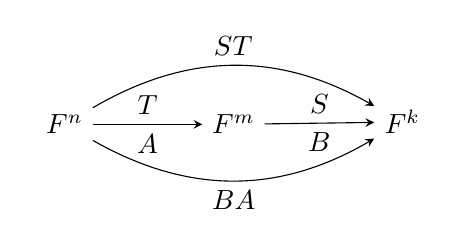
\begin{tikzpicture}
        \matrix (m) [matrix of math nodes, row sep=3em, column sep=4em, minimum width=2em]
        {F^n & F^m & F^k \\};
        \path[-stealth]
        (m-1-1) edge node [above] {$T$} node [below] {$A$} (m-1-2)
                edge [bend left] node [above] {$ST$} (m-1-3)
                edge [bend right] node [below] {$BA$} (m-1-3)
        (m-1-2) edge node [above] {$S$} node [below] {$B$} (m-1-3);
    \end{tikzpicture}
\end{center}

\begin{proposition}
    The standard matrix of the composition $ST: F^n \to F^k$ is the matrix multiplication $BA$, i.e., for all $\vec{x} \in F^n$,
    \[
        (ST)\vec{x} = B(A\vec{x}) = (BA)\vec{x}
    \]
\end{proposition}

\begin{proof}
    Let $\vec{x} \in F^n$ be a column matrix with entries $x_1, x_2, \cdots, x_n \in F$. Then $\vec{x}$ can be expressed as a linear combination of the standard basis vectors $\vec{e_1}, \vec{e_2}, \cdots, \vec{e_n}$:
    \[
        \vec{x} = x_1 \vec{e_1} + x_2 \vec{e_2} + \cdots + x_n \vec{e_n} = \sum_{i=1}^{n} x_i \vec{e_i}
    \]
    Consider the $j$-th column of $BA$, it is given by:
    \[
        (ST)\vec{e_j} = S(T(\vec{e_j})) = S(\vec{a_j}) = B\vec{a_j} = (BA)\vec{e_j}
    \]
    for all $j = 1, 2, \ldots, n$. This shows that the standard matrix of the composition $ST$ is indeed the matrix multiplication $BA$.
\end{proof}

\begin{remark}
    Note that $B$ is a $k \times m$ matrix and $A$ is an $m \times n$ matrix, so the matrix multiplication $BA$ is defined and results in a $k \times n$ matrix.
\end{remark}

\begin{remark}
    The matrix multiplication $BA$ can be computed as follows:
    \[
        BA = B\begin{bmatrix}
            | & | & & | \\
            \vec{a_1} & \vec{a_2} & \cdots & \vec{a_n} \\
            | & | & & |
        \end{bmatrix} = \begin{bmatrix}
            | & | & & | \\
            B\vec{a_1} & B\vec{a_2} & \cdots & B\vec{a_n} \\
            | & | & & |
        \end{bmatrix}
    \]
    where $\vec{a_i} = T(\vec{e_i})$ is the $i$-th column of the matrix $A$. Also, 
    \[
        B\vec{x} = x_1 \vec{b_1} + x_2 \vec{b_2} + \cdots + x_n \vec{b_n} = \sum_{i=1}^{n} x_i \vec{b_i}
    \]
    where $\vec{b_i} = B\vec{a_i}$ is the $i$-th column of the matrix $B$. Note that $B$ is a $k \times m$ matrix, and $\vec{x} \in F^m$. Thus, the matrix multiplication $B\vec{x}$ is defined and results in a column matrix in $F^k$.
\end{remark}

\newpage

\section{Elementary Row Operations}\index{Elementary Row Operations}

\begin{definition}[Elementary Row Operations]
    Let $A$ be an $m \times n$ matrix over a field $F$. An \emph{elementary row operation} on $A$ is one of the following operations:
    \begin{enumerate}
        \item Interchange two rows of $A$: $R_i \leftrightarrow R_j$.
        \item Multiply a row of $A$ by a nonzero scalar in $F$: $R_i \to \alpha R_i$ where $\alpha \in F \setminus \{0\}$.
        \item Add a scalar multiple of one row of $A$ to another row of $A$: $R_i \to R_i + \alpha R_j$ where $\alpha \in F$ and $i \neq j$.
    \end{enumerate}
    Each elementary row operation can be represented by \emph{left multiplication} of $A$ by an appropriate $m \times m$ matrix over $F$. Note that all of them are invertible linear maps from $F^{m \times n}$ to $F^{m \times n}$.
\end{definition}

For easier notations, we introduce the idea of matrix units, which is similar to the standard basis vectors $\vec{e_i}$.

\begin{definition}[Matrix Units]
    Let $m$ and $n$ be two positive integers and $F$ be a field. The \emph{matrix unit} $E_{ij}$ is the $m \times n$ matrix over $F$ with $1$ in the $(i,j)$-th position and $0$ elsewhere, i.e.,
    \[
        (E_{ij})_{kl} = \begin{cases}
            1 & \text{if } (k,l) = (i,j) \\
            0 & \text{otherwise}
        \end{cases}
    \]
    for all $1 \leq k \leq m$ and $1 \leq l \leq n$.

    It can also be defined as $E_{ij} = \vec{e_i} \hat{e_j} \in M_{m \times n} (F)$ where $\vec{e_i} \in F^m$ and $\vec{e_j}^T = \hat{e_j} \in F^n$ are the $i$-th and $j$-th standard basis vectors, respectively. The $\hat{e_j}$ is the row matrix with 1 in the $j$-th column and 0 anywhere else.
\end{definition}

\begin{remark}
    Note that for any $m \times n$ matrix $A$ over a field $F$, we have:
    \[
        \begin{split}
            A\vec{e_j} &= \text{the } j\text{-th column of } A \in F^n \\
            \hat{e_i}A &= \text{the } i\text{-th row of } A \in (F^m)^* \\
        \end{split}
    \]
    where $(F^m)^*$ is the set of all row matrices with $n$ entries in $F$. $\hat{e_i}$ is an element in $(F^m)^*$ for any $1 \leq i \leq m$. Then we have:
    \[
        a_{ij} = \hat{e_i} A \vec{e_j} = \text{the } (i,j)\text{-th entry of } A
    \]
\end{remark}

We can write the $E_{i,j}$ as:
\vspace{7ex}
\[
    E_{i,j} = \begin{bmatrix}
        0 & \cdots & 0 & \mypoint{herei}{0} & 0 & \cdots & 0 \\
        \vdots & \ddots & \vdots & \vdots & \vdots & \ddots & \vdots \\
        0 & \cdots & 0 & 0 & 0 & \cdots & 0 \\
        0 & \cdots & 0 & 1 & 0 & \cdots & \mypoint{herej}{0} \\
        0 & \cdots & 0 & 0 & 0 & \cdots & 0 \\
        \vdots & \ddots & \vdots & \vdots & \vdots & \ddots & \vdots \\
        0 & \cdots & 0 & 0 & 0 & \cdots & 0 \\
    \end{bmatrix}
\]
\begin{tikzpicture}[remember picture, overlay]
    \node[above=20pt of herei](textofhere1){the $i$-column};
    \draw[myarrow] (textofhere1) -- (herei);
    \node[right=20pt of herej](textofhere2){the $j$-row};
    \draw[myarrow] (textofhere2) -- (herej);
\end{tikzpicture}

Then we consider the row operations by using the matrix units.

\begin{proposition}
    The row operation $R_i \leftrightarrow R_j$ is a linear map where the standard matrix is $A_{R_i \leftrightarrow R_j} = I - E_{i,i} - E_{j,j} + E_{i,j} + E_{j,i}$.
\end{proposition}

\begin{proof}
    The linear map $T: F^n \to F^n$ is defined pointwisely. We can say the map is:
    \[
        \vec{e_k} \mapsto \begin{cases}
            \vec{e_j} & \text{if } k = i \\
            \vec{e_i} & \text{if } k = j \\
            \vec{e_k} & \text{if } k \neq i, j
        \end{cases}
    \]
    Then the standard matrix of $T$ is:
    \[
        A_{R_i \leftrightarrow R_j} = [\vec{e_1} \; \cdots \; \vec{e_j} \; \cdots \; \vec{e_i} \; \cdots \; \vec{e_n}] = I - E_{i,i} - E_{j,j} + E_{i,j} + E_{j,i}
    \]
    where $I$ is the $n \times n$ identity matrix.
\end{proof}

\begin{proposition}
    The row operation $R_i \to \alpha R_i$ where $\alpha \in F^x := F \setminus \{0\}$ is a linear map where the standard matrix is $A_{R_i \to \alpha R_i} = I + (\alpha - 1) E_{i,i}$.
\end{proposition}

\begin{proof}
    The linear map $T: F^n \to F^n$ is defined pointwisely. We can say the map is:
    \[
        \vec{e_k} \mapsto \begin{cases}
            \alpha \vec{e_i} & \text{if } k = i \\
            \vec{e_k} & \text{if } k \neq i
        \end{cases}
    \]
    Then the standard matrix of $T$ is:
    \[
        A_{R_i \to \alpha R_i} = [\vec{e_1} \; \cdots \; \alpha\vec{e_i} \; \cdots \; \vec{e_n}] = I + (\alpha - 1) E_{i,i}
    \]
    where $I$ is the $n \times n$ identity matrix.
\end{proof}

\begin{proposition}
    The row operation $R_i \to R_i + \alpha R_j$ where $\alpha \in F$ and $i \neq j$ is a linear map where the standard matrix is $A_{R_i \to R_i + \alpha R_j} = I + \alpha E_{i,j}$.
\end{proposition}

\begin{proof}
    The linear map $T: F^n \to F^n$ is defined pointwisely. We can say the map is:
    \[
        \vec{e_k} \mapsto \begin{cases}
            \vec{e_i} + \alpha \vec{e_j} & \text{if } k = i \\
            \vec{e_k} & \text{if } k \neq i
        \end{cases}
    \]
    Then the standard matrix of $T$ is:
    \[
        A_{R_i \to R_i + \alpha R_j} = [\vec{e_1} \; \cdots \; (\vec{e_i} + \alpha\vec{e_j}) \; \cdots \; \vec{e_n}] = I + \alpha E_{i,j}
    \]
    where $I$ is the $n \times n$ identity matrix.
\end{proof}

\newpage

\section{Dimensions of Vector Spaces}\index{Dimension of Vector Spaces}

\begin{definition}[Finite Dimensional Vector Spaces]
    A linear space $V$ over a field $F$ is said to be \emph{finite dimensional} if there exists a linear equivalence $T: V \to F^n$ for some positive integer $n$. In this case, we say that the dimension of $V$ is $n$, denoted $\dim_{F} V = n$ or simply $\dim V = n$.
\end{definition}

\begin{definition}[Infinite Dimensional Vector Spaces]
    A linear space $V$ over a field $F$ is said to be \emph{infinite dimensional} if $V$ is not finite dimensional.
\end{definition}

We have to proof if the dimension of a finite dimensional vector space is well-defined.

\begin{proposition}
    If there exists two linear equivalences $T: V \to F^m$ and $S: V \to F^n$, then $n = m$.
\end{proposition}

\begin{proof}
    Since $S$ is linear equivalence, it has a unique two-sided inverses $S^{-1}: F^n \to V$. Consider the composition of this map:
    \[
        TS^{-1}: F^n \to F^m
    \]
    Since $TS^{-1}$ is compositions of linear equivalences, it is also a linear equivalence. Mutantis mutandis, for the opposite direction.

    Now, we know that a linear equivalence between two finite-dimensional vector spaces. Then we have $\dim F^n = \dim F^m$ or $n = m$. Thus, the dimension of a finite dimensional vector space is well-defined.
\end{proof}

Graphically, we have the following commutative diagram:
\begin{center}
    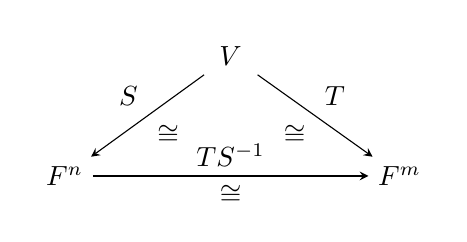
\begin{tikzpicture}
        \matrix (m) [matrix of math nodes, row sep=3em, column sep=4em, minimum width=2em]
        { & V & \\ F^n & & F^m \\};
        \path[-stealth]
        (m-1-2) edge node [above left] {$S$} node [below right] {$\cong$} (m-2-1)
                edge node [above right] {$T$} node [below left] {$\cong$} (m-2-3)
        (m-2-1) edge node [above] {$T S^{-1}$} node [below] {$\cong$} (m-2-3);
    \end{tikzpicture}
\end{center}

\begin{remark}
    In drawing commutative diagram, we can use $\xhookrightarrow{}$ to denote an injective linear map, $\twoheadrightarrow$ to denote a surjective linear map, and $\cong$ to denote a linear equivalence.
\end{remark}

\newpage

\section{Elementary Column Operations, Canonical Form and Rank}\index{Elementary Column Operations, Canonical Form and Rank}

\begin{definition}[Elementary Column Operations]
    Let $A$ be an $m \times n$ matrix over a field $F$. An \emph{elementary column operation} on $A$ is one of the following operations:
    \begin{enumerate}
        \item Interchange two columns of $A$: $C_i \leftrightarrow C_j$.
        \item Multiply a column of $A$ by a nonzero scalar in $F$: $C_i \to \alpha C_i$ where $\alpha \in F \setminus \{0\}$.
        \item Add a scalar multiple of one column of $A$ to another column of $A$: $C_i \to C_i + \alpha C_j$ where $\alpha \in F$ and $i \neq j$.
    \end{enumerate}
    Each elementary column operation can be represented by \emph{right multiplication} of $A$ by an appropriate $n \times n$ matrix over $F$. Note that all of them are invertible linear maps from $F^{m \times n}$ to $F^{m \times n}$.
\end{definition}

\begin{proposition}
    Any $m \times n$ matrix $A$ can be transformed into a matrix of the form $\begin{bmatrix}
        I_r & 0 \\
        0 & 0
    \end{bmatrix}$ by a finite sequence of elementary row and column operations on $A$, where $r$ is the rank of $A$.
\end{proposition}

\begin{center}
    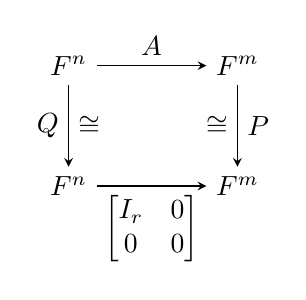
\begin{tikzpicture}
        \matrix (m) [matrix of math nodes, row sep=3em, column sep=4em, minimum width=2em]
        { F^n & F^m \\ F^n & F^m \\};
        \path[-stealth]
        (m-1-1) edge node [above] {$A$} (m-1-2)
                edge node [left] {$Q$} node [right] {$\cong$} (m-2-1)
        (m-1-2) edge node [right] {$P$} node [left] {$\cong$} (m-2-2)
        (m-2-1) edge node [below] {$\begin{bmatrix}
            I_r & 0 \\
            0 & 0
        \end{bmatrix}$} (m-2-2);
    \end{tikzpicture}
\end{center}

Note that $P$ is the product of a finite sequence of elementary row operation matrices and $Q$ is the product of a finite sequence of elementary column operation matrices. Both $P$ and $Q$ are invertible matrices. Thus, we have:
\[
    \begin{bmatrix}
        I_r & 0 \\
        0 & 0
    \end{bmatrix} = P A Q^{-1}
\]

\begin{definition}[Canonical Form of a Matrix]
    The matrix $\begin{bmatrix}
        I_r & 0 \\
        0 & 0
    \end{bmatrix}$ obtained from an $m \times n$ matrix $A$ by a finite sequence of elementary row and column operations on $A$ is called the \emph{canonical form} of $A$.    
\end{definition}

\begin{remark}
    The canonical form of a matrix defined above is also called the \emph{Smith Normal Form} or \emph{Normal Form} of a matrix.
\end{remark}

\begin{definition}[Rank of a Matrix]
    The \emph{rank} of an $m \times n$ matrix $A$ over a field $F$, denoted by $\text{rank}(A)$, is the number of leading 1's in the matrix $\begin{bmatrix}
        I_r & 0 \\
        0 & 0
    \end{bmatrix}$ obtained from $A$ by a finite sequence of elementary row and column operations on $A$.
\end{definition}

\begin{remark}
    The value $r$ is uniquely determined by $A$.
\end{remark}

% The graph of the canonical form of a matrix
\def\matriximg{%
    \begin{matrix}
        I_r & 0 \\
        0 & 0 
    \end{matrix}
}

\begin{proposition}
    Let $A$ be an $n \times n$ matrix over a field $F$. Then the following statements are equivalent:
    \[
        A \text{ is invertible } \iff m \left\{\left[\vphantom{\matriximg}\right.\right.\kern-2\nulldelimiterspace
        \underbrace{\matriximg}_{\text{\normalsize $n$}}\kern-\nulldelimiterspace\left.\vphantom{\matriximg}\right] \text{ is invertible } \iff \text{rank}(A) = m = n \iff \begin{bmatrix}
            I_r & 0 \\
            0 & 0
        \end{bmatrix} = I_n
    \]
\end{proposition}

\begin{proposition}
    Let $A$ be an $m \times n$ matrix over a field $F$. Then the following statements are equivalent:
    \[
        \text{rank}(A) = n \iff A \text{ has a right inverse } \iff A \text{ is injective } \iff \begin{bmatrix}
            I_r & 0 \\
            0 & 0
        \end{bmatrix} = \begin{bmatrix}
            I_n \\
            0
        \end{bmatrix}
    \]
\end{proposition}

\begin{proposition}
    Let $A$ be an $m \times n$ matrix over a field $F$. Then the following statements are equivalent:
    \[
        \text{rank}(A) = m \iff A \text{ has a left inverse } \iff A \text{ is surjective } \iff \begin{bmatrix}
            I_r & 0 \\
            0 & 0
        \end{bmatrix} = \begin{bmatrix}
            I_m & 0
        \end{bmatrix}
    \]
\end{proposition}

\begin{proposition}
    For every $\vec{b}$, $\begin{bmatrix}
        I_r & 0 \\
        0 & 0
    \end{bmatrix} \vec{x} = \vec{b}$ has a unique solution.
\end{proposition}

Linear Algebra is the study of linear map between two finite dimensional vector spaces.

\begin{center}
    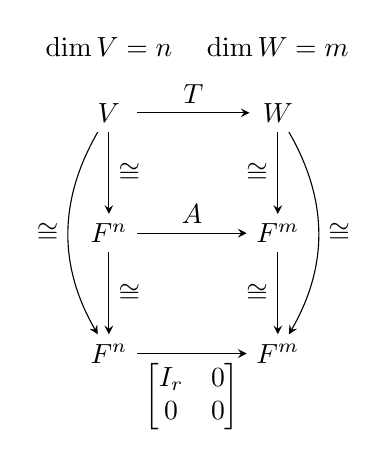
\begin{tikzpicture}
        \matrix (m) [matrix of math nodes, row sep=3em, column sep=4em, minimum width=2em]
        { V & W \\ F^n & F^m \\ F^n & F^m \\};
        \path[-stealth]
        (m-1-1) edge node [above] {$T$} (m-1-2)
                edge node [right] {$\cong$} (m-2-1)
                edge [bend right] node [left] {$\cong$} (m-3-1)
        (m-1-2) edge node [left] {$\cong$} (m-2-2)
                edge [bend left] node [right] {$\cong$} (m-3-2)
        (m-2-1) edge node [above] {$A$} (m-2-2)
                edge node [right] {$\cong$} (m-3-1)
        (m-2-2) edge node [left] {$\cong$} (m-3-2)
        (m-3-1) edge node [below] {$\begin{bmatrix}
            I_r & 0 \\
            0 & 0
        \end{bmatrix}$} (m-3-2);
        \path (m-1-1) node [above=10pt of m-1-1] {$\dim V = n$};
        \path (m-1-2) node [above=10pt of m-1-2] {$\dim W = m$};
    \end{tikzpicture}
\end{center}

The bended arrows denote the trivialisation of the vector spaces and the bottom arrow denotes the canonical matrix representation of the linear map $T$.

\chapter{Linear Spaces}

\epigraph{Babies have to survive, so they have the strong desire to learn stuffs. You think you are not good at math because you don't have the strong desire to learn math.}{Guowu Meng}

\section{Linear Subspaces, Kernels and Images}\index{Linear Subspaces, Kernels and Images}

\begin{definition}[Linear Subspaces]
    Let $W$ be a linear space over $F$ and $V$ is a subset of $W$, denoted as $V \subset W$. $V$ is a \emph{(linear) subspace} of $W$ if $V$, with $+$ and $\cdot$ inherited from those of $W$, is a linear space.
\end{definition}

\begin{proposition}
    Let $V \subset W$. $V$ is a subspace of $W$ if and only if $V$ is not empty and $V$ is closed under $+$ and $\cdot$.
\end{proposition}

\begin{definition}[Kernels]
    Let $f : V \to W$ be a linear map. The \emph{kernel} of $f$, denoted as $\ker f$, is defined as 
    \[
        \ker f \overset{\text{def}}{=\joinrel=} f^{-1}(0_W) = \{ v \in V \mid f(v) = 0_W \}
    \]
\end{definition}

\begin{example}
    Let $f : V \to W$ be a linear map. $\ker f$ is a subspace of domain of $f$, i.e., $V$.
    
    First, we have $0_V \in \ker f$, as $f(0_V) = 0_W$, so $\ker f$ is not empty.

    Then we consider $\alpha_1, \alpha_2 \in F$ and $v_1, v_2 \in \ker f$, we have
    \[
        f(\alpha_1 v_1 + \alpha_2 v_2) = \alpha_1 f(v_1) + \alpha_2 f(v_2) = \alpha_1 (0_W) + \alpha_2 (0_W) = 0_W
    \]
    The first equality due to the linearity of $f$ and the second is due to $v_i \in \ker f$.
\end{example}

\begin{definition}[Images]
    Let $f : V \to W$ be a linear map. The \emph{image} of $f$, denoted by $\Im f$, is defined as 
    \[
        \Im f \overset{\text{def}}{=\joinrel=} \{ f(v) \mid v \in V \} \subset W
    \]
\end{definition}

\begin{example}
    Let $f : V \to W$ be a linear map. $\Im f$ is a subspace of codomain of $f$, i.e., $W$.

    First, we have $f(0_V) = 0_W \in \Im f$, so $\Im f$ is not empty.

    Then we consider $\alpha_1, \alpha_2 \in F$ and $f(v_1), f(v_2) \in \Im f$. We have 
    \[
        \alpha_1 f(v_1) + \alpha_2 f(v_2) = f(\alpha_1 v_1 + \alpha_2 v_2) \in \Im f
    \]
    The equality is due to the linearity of $f$.
\end{example}

\begin{example}
    Let $W$ be a linear space over a field $F$ and $\{V_\alpha\}_{\alpha \in I}$ be the family of subspaces of $W$ indexed by the element in the index set $I$. Then $\bigcap_{\alpha \in I} V_\alpha$ is also a subspace of $W$.

    First, we have $0_W \in V_\alpha$ for all $\alpha \in I$, so $0_W \in \bigcap_{\alpha \in I} V_\alpha$. Thus, $\bigcap_{\alpha \in I} V_\alpha$ is not empty.

    Then we consider $\alpha_1, \alpha_2 \in F$ and $v_1, v_2 \in \bigcap_{\alpha \in I} V_\alpha$. We have $v_1, v_2 \in V_\alpha$ for all $\alpha \in I$. Thus, $\alpha_1 v_1 + \alpha_2 v_2 \in V_\alpha$ for all $\alpha \in I$. This shows that $\alpha_1 v_1 + \alpha_2 v_2 \in \bigcap_{\alpha \in I} V_\alpha$.
\end{example}

Then we consider the duality of the intersection and union of subspaces. Whether the union of two subspaces is still a subspace? Unfortunately, the answer is no in general case. However, we have the following proposition.

\begin{proposition}
    Let $W$ be a linear space over a field $F$ and consider the family of subspaces $\{V_\alpha\}_{\alpha \in I}$. Then $\bar{\bigcup_{\alpha \in I} V_\alpha}$ is a subspace of $W$ where $\bar{\bigcup_{\alpha \in I} V_\alpha}$ is the completion of $\bigcup_{\alpha \in I} V_\alpha$ under linear combinations. We call $\bar{\bigcup_{\alpha \in I} V_\alpha}$ the \emph{sum} of the subspaces $\{V_\alpha\}_{\alpha \in I}$, denoted by $\sum_{\alpha \in I} V_\alpha$.
\end{proposition}

\newpage

\section{Linear Span and Linear Independence}\index{Linear Span and Linear Independence}

\begin{definition}[Linear Span]
    Let $W$ be a linear space over a field $F$ and $S \subset W$. The \emph{(linear) span} of $V$, denoted by $\text{span}_F (S)$ or simply $\span S$ or $\bar{S}$, is defined as the completion of $S$ inside $W$ under linear combinations.
\end{definition}

\begin{corollary}
    $\span S$ can also be defined as the intersection of all subspaces of $W$ containing $S$, which is the smallest subspace of $W$ containing $S$. It can be written as:
    \[
        \span S = \bigcap_{V \in I} V \subset V \quad \text{where } I = \{ V \subset W \mid V \text{ is a subspace of } W \text{ and } S \subset V \}
    \]
\end{corollary}

\begin{remark}
    Note that $I$ is not empty as $W \in I$. Thus, $\span S$ is well-defined. $W$ is the largest subspace of itself and $\{0_W\}$ is the smallest subspace of $W$.
\end{remark}

\begin{proposition}
    Let $W$ be a linear space over a field $F$ and $S \subset W$. Then 
    \[
        \span S = \left\{ \sum_{i=1}^{n} \alpha_i s_i \mid n \in \mathbb{N}, \alpha_i \in F, s_i \in S \right\}
    \]
    Note that the summation is a finite summation.
\end{proposition}

\begin{definition}[Linear Independences]
    Let $W$ be a linear space over a field $F$ and $V_1, \cdots, V_k$ be subspaces of $W$. The subspaces $V_1, \cdots, V_k$ are said to be \emph{linearly independent} if $V_i \neq \{0_W\}$ for all $i$ and there is one and only one way to split $0_W \in W$ as a sum of vectors from each $V_i$, i.e., if $v_i \in V_i$ for all $i$ and $\sum_{i=1}^{k} v_i = 0_W$, then $v_i = 0_W$ for all $i$.
\end{definition}

\begin{proposition}
    $v_1, v_2, \cdots, v_k \in W$ are independent if the subspaces $\span{v_1}$, $\span{v_2}$, $\cdots$, $\span{v_k}$ are linearly independent.
\end{proposition}

\begin{proposition}
    $v_1, v_2, \cdots, v_k \in W$ are linearly independent if and only if there is one and only one way to write $0_W \in W$ as the combination of $v_1, \cdots, v_k$ with coefficients in $F$, i.e., the equation 
    \[
        \alpha_1 v_1 + \cdots + \alpha_k v_k = 0_W
    \]
    has only  the trivial solution, i.e., $\alpha_i = 0$ for all $i$.
\end{proposition}

Given a linear space $V$ over a field $F$. We define the order set $S := \{\vec{v_1}, \vec{v_2}, \cdots, \vec{v_n}\} \subseteq V$. The order set $S$ forms a linear map $\phi_S: F^n \to V$ defined by:
\[
    \phi_S(\vec{x}) = \phi_S\left(\begin{bmatrix}
        x_1 \\
        x_2 \\
        \vdots \\
        x_n
    \end{bmatrix}\right) = x_1 \vec{v_1} + x_2 \vec{v_2} + \cdots + x_n \vec{v_n} = \sum_{i=1}^{n} x_i \vec{v_i}
\]

\begin{proposition}
    The order set $S := \{\vec{v_1}, \vec{v_2}, \cdots, \vec{v_n}\} \subseteq V$ is said to be \emph{linearly independent} if and only if the linear map $\phi_S: F^n \to V$ defined above is injective.
\end{proposition}

\begin{proposition}
    The order set $S := \{\vec{v_1}, \vec{v_2}, \cdots, \vec{v_n}\} \subseteq V$ is said to be a \emph{spanning set} of $V$ if and only if the linear map $\phi_S: F^n \to V$ defined above is surjective.
\end{proposition}

\newpage

\section{Group Actions}\index{Group Actions}

\begin{definition}[Group Actions]
    Let $G$ be a group and $X$ be a set. A \emph{(left) group action} of $G$ on $X$ is a map $\cdot : G \times X \to X$, $(g, x) \mapsto g \cdot x$, such that for all $g_1, g_2 \in G$ and $x \in X$, the following properties hold:
    \begin{enumerate}
        \item Compatibility: $(g_1 g_2) \cdot x = g_1 \cdot (g_2 \cdot x)$.
        \item Identity: $e \cdot x = x$ where $e$ is the identity element of $G$.
    \end{enumerate}
\end{definition}

Consider rotation in a plane. It is a group action of the group $SO(2)$ on the set $\mathbb{R}^2$.
\[
    g = \begin{pmatrix}
        \cos{\theta} & -\sin{\theta} \\
        \sin{\theta} & \cos{\theta}
    \end{pmatrix}
\]

Then we have the following group action:
\begin{center}
    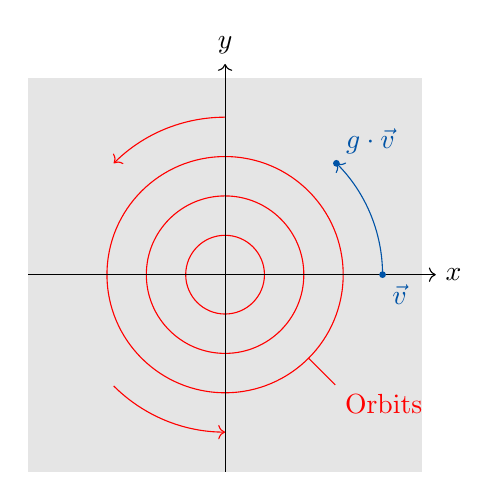
\begin{tikzpicture}
        \draw[draw=none,fill=gray!20] (-2.5,-2.5) rectangle (2.5,2.5);
        \draw[red] (0,0) circle (1.5cm);
        \draw[red] (0,0) circle (1cm);
        \draw[red] (0,0) circle (0.5cm);
        \draw[red] (1.06066,-1.06066) -- (1.4,-1.4) node[below right]{Orbits};

        \filldraw[ocre] (1.414,1.414) circle (1pt) node[above right]{$g \cdot \vec{v}$};
        \draw[->] (-2.5,0) -- (2.5cm + 5pt,0) node[right]{$x$};
        \draw[->] (0,-2.5) -- (0,2.5cm + 5pt) node[above]{$y$};
        \filldraw[ocre] (2,0) circle (1pt) node[below right]{$\vec{v}$};
        \draw[->,ocre] (2,0) arc[start angle=0,end angle=45,radius=2];
        \draw[->,red] (0,2) arc[start angle=90,end angle=135,radius=2];
        \draw[->,red] (-1.414,-1.414) arc[start angle=225,end angle=270,radius=2];
    \end{tikzpicture}
\end{center}

\begin{definition}[Orbits]
    Let $G$ be a group acting on a set $X$. The \emph{orbit} of the action through a point $x \in X$, denoted as $G \cdot x$, is defined as the set of points in $X$ that can be reached from $x$ by the action of elements of $G$, i.e., 
    \[
        G \cdot x = \{g \cdot x \mid g \in G\}
    \]
\end{definition}

\begin{definition}[Partition]
    A \emph{partition} of a set $X$ is a collection of non-empty, disjoint subsets of $X$ whose union is $X$. The partition of the set $X$ is the same as an equivalence relation on $X$.
\end{definition}

\begin{proposition}
    Orbits give a partition of the set $X$, i.e., $X$ can be expressed as the disjoint union of its orbits. The orbits of the action are the equivalence classes of the equivalence relation.
\end{proposition}

\begin{proposition}
    Let $f : X \to Y$ be a map between two sets $X$ and $Y$. Then $f$ defines a partition of $X$ by the equivalence relation. The equivalence classes are the preimages of points in $Y$, i.e., $f^{-1}(y)$ for each $y \in Y$.
\end{proposition}

\newpage

\begin{example}
    Let $V$ be a subspace of a linear space $W$ over a field $F$. We know $(V, +)$ is an abelian group. Then we have the group action of $V$ on $W$ defined by: $(v, w) \mapsto v + w \in W$ \quad for all $v \in V, w \in W$
    We know that $(v_1 + v_2) + w = v_1 + (v_2 + w)$ and $0_V + w = w$ for all $v_1, v_2 \in V$ and $w \in W$. Thus, it is a group action. 
    
    \begin{center}
        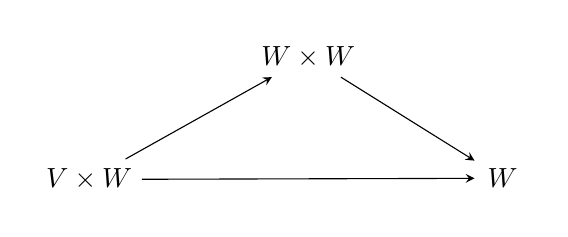
\begin{tikzpicture}
            \matrix (m) [matrix of math nodes, row sep=3em, column sep=4em, minimum width=2em]
            { & W \times W & \\ V \times W & & W \\};
            \path[-stealth]
            (m-1-2) edge (m-2-3)
            (m-2-1) edge (m-2-3)
                    edge (m-1-2);
        \end{tikzpicture}
    \end{center}
\end{example}

This group action defines this equivalence relation on $W$:
\[
    w_1 \sim w_2 \iff \exists w_2 - w_1 \in V
\]

\newpage

\section{Quotient Spaces}\index{Quotient Spaces}

We consider the duality of the subspace, i.e., the quotient space.

\begin{definition}[Quotient Spaces]
    % Let $W$ be a linear space over a field $F$ and $V$ be a subspace of $W$. The \emph{quotient space} of $W$ by $V$, denoted by $W / V$, is defined as the set of equivalence classes of $W$ under the equivalence relation defined by the group action of $V$ on $W$, i.e., the set of $V$-equivalence classes. The equivalence class of an element $w \in W$ is denoted by $w + V$ and is called a \emph{coset} of $V$ in $W$. Thus, we have
    % \[
    %     W / V = \{ w + V \mid w \in W \}
    % \]
    % where 
    % \[
    %     w + V = \{ w + v \mid v \in V \}
    % \]
    % for each $w \in W$.
\end{definition}

Consider a linear space $W$ over a field $F$.
\begin{center}
    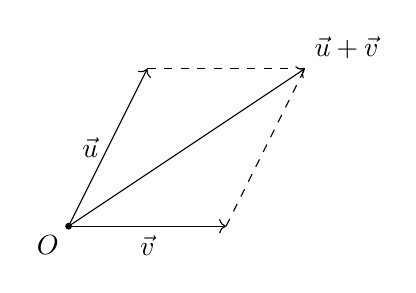
\begin{tikzpicture}
        \filldraw (0,0) circle (1pt) node [below left] {$O$};
        \draw[->] (0,0) -- (2,0) node [midway, below] {$\vec{v}$};
        \draw[->] (0,0) -- (1,2) node [midway, left] {$\vec{u}$};
        \draw[dashed] (1,2) -- (3,2);
        \draw[dashed] (2,0) -- (3,2);
        \draw[->] (0,0) -- (3,2) node [above right] {$\vec{u} + \vec{v}$};
    \end{tikzpicture}
\end{center}
Then consider a subspace $V \in W / V$.
\begin{center}
    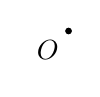
\begin{tikzpicture}
        \filldraw (0,0) circle (1pt) node [below left] {$O$};
        \draw[dashed,fill=gray!20] ;
    \end{tikzpicture}
\end{center}


%----------------------------------------------------------------------------------------

\end{document}
